\section{Numerical Comparisons}
\label{sec:experiments}

\subsection{MS (Multi-start)}
\label{compare:ms}

Multi-start techniques form a family of heuristic global optimization algorithms. These techniques work in a two-phase
process. In the first global phase, starting points are sampled in the feasible region or domain $\mathcal{S}$ of the
objective function. The most naive implementation of the global phase is to simply perform a uniform sampling of $\mathcal{S}$.
Some members of this family of algorithms utilize sophisticated heuristics to generate starting points such as the
Scatter Search technique.

The local phase of multi-start algorithms use the starting points from the global phase to perform a local optimization
using one of the many algorithms for local optimization. Multi-start algorithms alternate between the global and local
phases until a solution is found \cite{Ugray2007ScatterSA}.

The hardest part of divising an efficient Multi-start method is the selection of an appropriate stopping rule.
Variations in the literature range from several addhoc holes to Bayesian stoppic rules. For the sake of comparison
we utilize a double-box stopping rule [cite box-cstr here].

Let $m(\mathcal{S})$ be the Lebesque measure of the search region $\mathcal{S}$. Since the local search method is
deterministic, in the limit of $n\rightarrow \infty$ runs of the local search method, the algorithm will converge
to $w$ unique local minima. Each local minimum $\vect{x}_i^\star \in\mathcal{S}$ has an associated region of
attraction $A_i$ defined as

$$
A_i := \left\lbrace \vect{x} : \vect{x}\in\mathcal{S}, \texttt{LS}(\vect{x}) = \vect{x}_i^\star \right\rbrace.
$$

Since $\mathcal{S}$ contains $w$ local minima, and the $A_i\cap A_j=\emptyset$, $A_i$ partitions $\mathcal{S}$ i.e.,

$$
\bigcup_{i=1}^w A_i = \mathcal{S}.
$$

Furthermore, if $m(A_i)$ denotes the Lebesque measure of $A_i$, then

$$
m(\mathcal{S}) = \sum_{i=1}^w m(A_i).
$$

If some initial point $\vect{x}_0 \sim \text{Uniform}(\mathcal{S})$, then the probability of $\vect{x}_0$ begin contained
in $A_i$ is simply

$$
P(\vect{x}_0 \in A_i) = \frac{m(A_i)}{m(\mathcal{S})}.
$$

The double-box stopping rule is based on the idea that we want to ensure that all $A_i$ are sampled in $\mathcal{S}$, but
additional sampling results in uncessary computation. Define $C$ has a relative measure of the coverage after the discovery
of $w$ local minima, as

\begin{equation}\label{eq:coverage}
C = \sum_{i=1}^w \frac{m(\mathcal{A}_i)}{m(\mathcal{S})}.
\end{equation}

A sensible heuristic is to stop when $C\longrightarrow 1$. The quantity inside the summation of \cref{eq:coverage} is
not calculatable in practice, but as $w\rightarrow \infty$, we approximate it with

\begin{equation}\label{eq:cov_approx}
C \approx \sum_{i=1}^w \frac{L_i}{L},
\end{equation}

where $L_i$ is the number of starting points of the LS which converged to the local minimizer $\vect{x}_i$, and
$L$ is the total of initial points so far. The quantity in \cref{eq:cov_approx} is equal to 1 by definition, so another
means must be determined. Construct a region $\mathcal{S}_2$ such that $\mathcal{S}\subset \mathcal{S}_2$ and 
$m(\mathcal{S}_2) = 2\cdot m(\mathcal{S})$. For each iteration, we sample from $\mathcal{S}_2$ until we have a point in
$\mathcal{S}$, in other words points in $A_0 = \mathcal{S}_2 \setminus \mathcal{S}$ are discared. Also let
$L_0$ denote the number of sampled points in $A_0$. The total count of sampled points is now given by

$$
L = L_0 + \sum_{i=1}^w L_i,
$$

and the relative coverage $C$ is now

$$
C = \frac{1}{m(\mathcal{S})} \sum_{i=1}^w m(A_i) = 2\sum_{i=1}^w \frac{m(A_i)}{m(\mathcal{S}_2)}
$$

and finally we can approximate relative coverage with

$$
C \approx \frac{2}{L}\sum_{i=1}^w L_i
$$

After $n$ iterations, let $M_n$ denote the number of points in $\mathcal{S}_2$, and $n$ are in $\mathcal{S}$. Then define
$\delta_n := n / M_k$ which has an expectation which in the limit of large $n$

$$
\left\langle \delta \right\rangle_n = \frac{1}{n}\sum_{i=1}^n \delta_i \longrightarrow
\frac{m(\mathcal{S})}{m(\mathcal{S}_2)} = \frac{1}{2}
$$

The variance is $\sigma_n^2(\delta) = \left\langle \delta^2\right\rangle_n - \left\langle\delta\right\rangle^2_n$ which
$\longrightarrow 0$ as $n\longrightarrow \infty$. Finally, the double-box rule is

\subsubsection*{Double-box stopping rule:}

\hfill\\

\textbf{(1)} Continue iterating if new minima are found. \textbf{(2)} If no new minima are found, let $\sigma_\text{last}(\delta)$ be the s.t.d. at the last iteration
at which a minimum was found. Contnue iterating while

\begin{equation}\label{eq:double-box-rule}
    \sigma^2(\delta) < \rho \sigma^2_{\text{last}}(\delta)
\end{equation}

where $\rho \in (0,1)$ is a paramter that performs exhaustive search when $\rho$ is close to 0 and emphasises less iterations
when $\rho$ is close to 1.

\subsubsection*{Constructing $\mathcal{S}_2$ from $\mathcal{S}$:}

\hfill\\

In order to apply the double-box stopping rule, we need to construct the box region $\mathcal{S}_2$ such that
$m(\mathcal{S}_2) = 2\cdot m(\mathcal{S})$. Suppose $\mathcal{S}\in\Real^n$, then we can scale the bounds of $\mathcal{S}
= [l_1, u_1] \times \cdots [l_n, u_n]$ 
by $2^{1/n}$, i.e.,

$$
l_i^{(2)} = l_i - \frac{1}{2}\left( 2^{1/n} - 1\right)\left( u_i - l_i \right)\text{ for } i = 1,\ldots n
$$
$$
u_i^{(2)} = u_i + \frac{1}{2}\left( 2^{1/n} - 1\right)\left( u_i - l_i \right)\text{ for } i = 1,\ldots n
$$


\begin{algorithm}
\setstretch{1.4}
\caption{Multi-start}\label{algo:multistart}
\vspace{8pt}
\nosemic
\SetAlgoLined
\KwIn{
    $f:\mathcal{S}\longleftarrow \Real,
    \nabla f,
    \mathcal{S},
    \tau, \rho, \epsilon_s, N
    $
}

$\mathcal{S}_2 \longleftarrow \texttt{scale}(\mathcal{S}, 2) $ \;

$M_n \longleftarrow 0$ \;

x\_minima $ \longleftarrow \left\lbrace \: \right\rbrace$ \;
deltas $ \longleftarrow \left\lbrace \: \right\rbrace$ \;

f\_best $\longleftarrow \infty$ \;

\For{ $n \in \left\lbrace 1,\ldots, N\right\rbrace$ } {

    \While{true} {
        $\vect{x} \longleftarrow \texttt{sample}(\mathcal{S}_2) $ \;

        $M_n \longleftarrow M_n + 1$ \;

        \If{ $\vect{x} \in \mathcal{S}$ } {
            \textbf{break} \;
        }
    }

    $\vect{x}_{ls} \longleftarrow \texttt{LS}( f, \vect{x}, \nabla f ) $\;

    \If{ $\vect{x}_{ls} \not\in \mathcal{S}$ } {
        \textbf{continue} \;
    }

    $\Delta = n / M_n$ \;
    deltas$.\texttt{push}(\delta)$ \;

    f\_ls $\longleftarrow f(\vect{x}_{ls}) $ \;

    $\sigma^2 \longleftarrow \texttt{var}(\text{deltas})$ \;

    \If{ f\_ls < f\_best } {
        f\_best = f\_ls \;
        $\vect{x}^\star \longleftarrow \vect{x}_{ls}$ \;
    }

    \If{ $\vect{x}^\star \not\in \text{x\_minima}$ } {
        $\sigma^2_{prev} \longleftarrow \sigma^2$ \;
        x\_minima$.\texttt{push}( \vect{x}_{ls} )$ \;
    } 
    \uElse {

    \Comment{Check double-box stop cond.}
    \If { $\sigma^2 < \rho \cdot \sigma^2_{prev}$ } {
        \Return{ $\vect{x}^\star$ }
    }

}
}
\;
\KwOut{`failed to reach tolerance in $N$ iterations'}
\Return{ $\vect{x}^\star$ }

%\Return{$\vect{x}$}

\end{algorithm}
%\begin{algorithm}
%\setstretch{1.4}
%\caption{Multi-start with double-box stopping rule}\label{algo:multistart}
%\vspace{8pt}
%\nosemic
%\SetAlgoLined
%\KwIn{$f:\mathcal{S} \longrightarrow \Real, \nabla f, \mathcal{S}, N, \epsilon_s, \tau, \gamma$}

%$f^\star \longleftarrow \infty$\;

%\;

%\For{$n\in \left\lbrace 1,\ldots, N\right\rbrace$}{
%$\vect{x}_0 \longleftarrow \mathrm{Uniform}\left(\mathcal{S}\right)$ \Comment*{random sample init. point}

%$x_l = \texttt{steepest\_descent}(f, \nabla f, \vect{x}_0, \tau)$ \;

%\If{$f(\vect{x}_l) \leq f^\star$}{
%    $f^\star \longleftarrow f(\vect{x}_l)$ \;
%    
%    $\vect{x}^\star \longleftarrow \vect{x}_l$ \;
%}

%\uIf{$n=0$}{
%    $f^\star_s \longleftarrow C$ \Comment*{$0< C \in\Real$ to prevent 0}
%    $f^\star_s^{(0)} \longleftarrow f_s^\star$ \;
%} \uElse{
%    $f^\star_s^{(0)} \longleftarrow f^\star_s$ \;
%    $f^\star_s = \gamma f^\star + (1-\gamma)f^\star_s^{(0)}$
%    \;
%    \Comment{Stop when smoothed improvement reaches 0}
%    $\Delta_s = f^\star_s^{(0)} - f^\star_s$ \;
%    
%    \Comment{Check stop condition}
%    \If{ $\Delta_s \leq \epsilon_s$}{
%        \KwOut{Solution found $\vect{x}^\star$}
%    }
%}

%\;
%\KwOut{Failed to find solution in $N$ iterations, $\vect{x}^\star$}\;
%}
%\end{algorithm}

\subsection{DE (Differential Evolution)}
\label{compare:de}

Differential Evolution is global, gradient-free stochastic optimization algorithm. This population-based method mutates
each solution candidate by mixing the solution with other members of the  population \cite{storn}.
We use

\noindent\texttt{scipy.optim.differential\_evolution} for comparison.

\subsection{BH (Basin Hopping)}
\label{compare:bh}

Basin-hopping is another two-phase global optimization algorithm inspired by energy minimization of clusters of atoms \cite{wales}.
We use

\noindent\texttt{scipy.optimize.basinhopping} for comparison.


\subsection{Evaluation metrics}

In \cref{metric1} and \cref{metric2}, we consider a global minimum to have been found once 
$\left|\hat{\vect{x}}_j - \vect{x}^\star_i\right|_2 \leq \tau = 10^{-4}$. Over a total of $M$ trials, let
$k_i$ denote the number of runs to find all $w$ global minima on the $i$-th trial.

\subsubsection{Metric 1: Number of runs required to find all global minima}\label{metric1}

One method to compare various global optimization methods is to calculate the number of runs required to find all
global minima for a given benchmark, averaged over $M$ runs, divided by the number of minima $w$.
We can define metric $\xi_1$ with \cref{eq:metric1}.

\begin{equation}\label{eq:metric1}
\xi_1 = \frac{1}{wM} \sum_{i=1}^M k_i 
\end{equation}

\subsubsection{Metric 2: Number of function evaluations to find all global minima}\label{metric2}

Different optimization methods use evaluations of $f$ and $\nabla f$ in very different ways. Methods that utilize a
local search will incur large numbers of calls to these functions inside of their inner loops. Examining the average
number of these evaluations to find all global minima of a given benchmark function is a good way to compare the
computational cost of various methods. Similiar to \cref{metric1}, we average the number of required calls over
$M$ trials. Furtheremore, to make comparisons accross different benchmakrs, divide by the number of minima $w$.
Suppose it takes $k_i$ runs to find all $w$ global minima, on the $i$-th trial, 
where $i\in\left\lbrace 1,\ldots, M\right\rbrace$. We define metric $\xi_2$ with \cref{eq:metric2}.

\begin{equation}\label{eq:metric2}
\xi_2 = \frac{1}{wM}\sum_{i=1}^M \sum_{j=1}^{k_i} \left( n(f_{ij}) + n(\nabla_{ij}) \right),
\end{equation}

where $n(f_{ij})$ and $n(\nabla_{ij})$ denotes the number of evaluations of the function $f$ and its Jacobian respectively,
incurred during the $j$-th run of the $i$-th trial.

\begin{table}
    \center
    \caption{Finding all minima}
    \label{table:compare-all}
    \footnotesize
    \setstretch{1.4}
    \begin{tabular}{cc|ccccc}
        Benchmark $f$ & Method & $\overline{n(f_{ij})}$ & $\overline{n(\nabla_{ij})}$ & $\Delta t$ (ms) & $\xi_1$ & $\xi_2$  \\
        \hline
RB  & BH & 6590.6 & 2045.5 & 458 & 1.0 & 4318.0 \\
 & DE & 3895.5 & 0.0 & 232 & 1.0 & 1948.0 \\
 & MS & 1031.4 & 981.5 & 90 & 1.0 & 1006.0 \\
 & SA & 631.8 & 220.0 & 15 & 1.0 & 426.0 \\
\hline
GP  & BH & 19532.9 & 6181.6 & 1279 & 1.0 & 12857.0 \\
 & DE & 966.4 & 0.0 & 63 & 1.0 & 483.0 \\
 & MS & 608.2 & 575.2 & 73 & 1.0 & 592.0 \\
 & SA & 1056.3 & 378.4 & 48 & 1.6 & 717.0 \\
\hline
BR  & BH & 20369.5 & 6665.0 & 1422 & 1.8 & 4506.0 \\
 & DE & 9163.4 & 0.0 & 569 & 3.1 & 1527.0 \\
 & MS & 1437.3 & 1293.0 & 139 & 2.02 & 455.0 \\
 & SA & 2761.4 & 946.5 & 77 & 1.57 & 618.0 \\
\hline
H3  & BH & 8817.8 & 2177.6 & 580 & 1.0 & 5498.0 \\
 & DE & 22736.6 & 0.0 & 1625 & 16.15 & 11368.0 \\
 & MS & 444.9 & 418.3 & 61 & 1.0 & 432.0 \\
 & SA & 570.2 & 207.8 & 34 & 1.1 & 389.0 \\
\hline
H6  & BH & 22008.6 & 3132.0 & 1267 & 1.0 & 12570.0 \\
 & DE & 22513.6 & 0.0 & 1807 & 4.5 & 11257.0 \\
 & MS & 876.7 & 845.6 & 215 & 1.0 & 861.0 \\
 & SA & 629.1 & 252.2 & 72 & 1.45 & 441.0 \\
    \end{tabular}
\end{table}

\begin{figure}
    \center
    \caption{Finding all minima}
    \label{fig:compare1}
    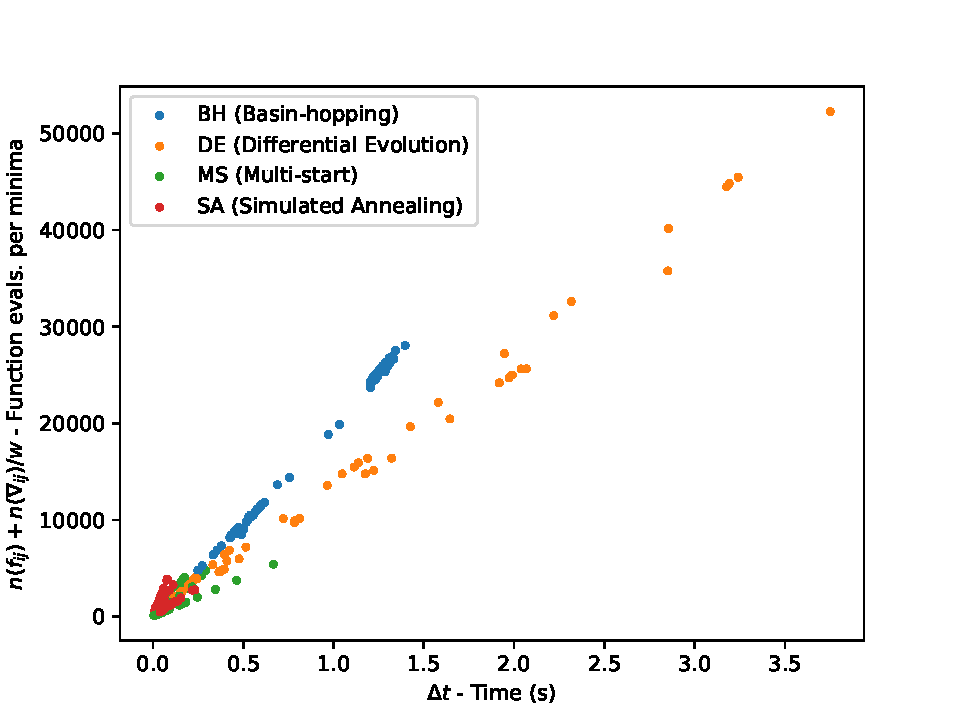
\includegraphics[scale=0.5]{figures/compare1-1.pdf}
\end{figure}

\begin{figure}
    \center
    \caption{Finding all minima (log scale)}
    \label{fig:compare-log}
    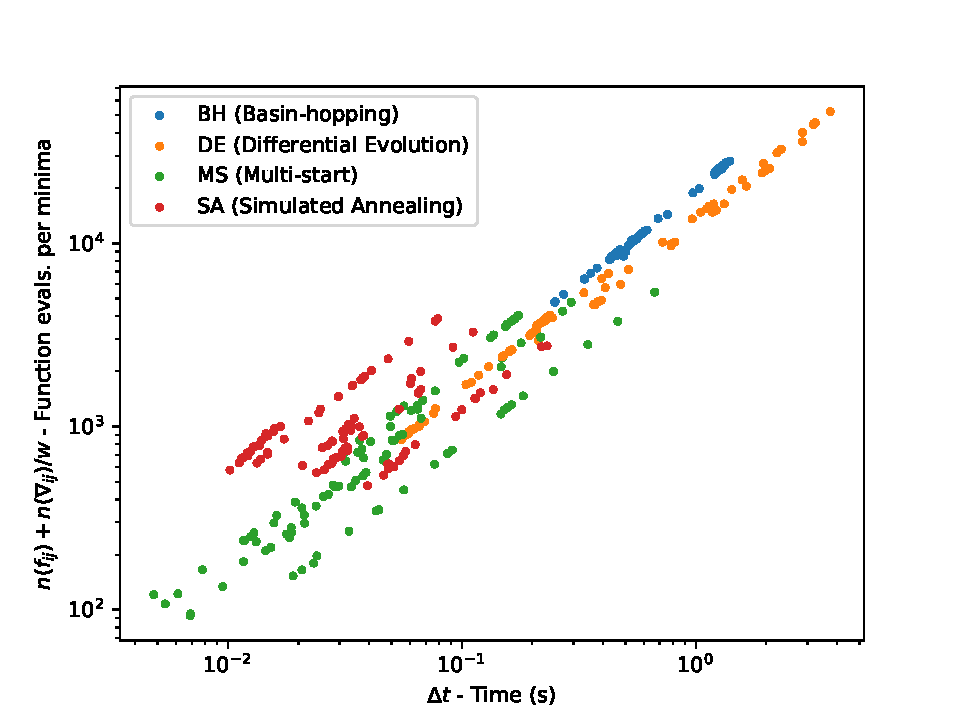
\includegraphics[scale=0.5]{figures/compare1-2.pdf}
\end{figure}

\Cref{table:compare-all} shows that, in terms of average running time $\overline{\Delta t}$,
our implementation of Simulated Annealing outperformed all other methods on every benchmark. Multi-start is arguably
the second best performing method. \Cref{fig:compare1} shows that SA has generally faster running time. Mutli-start
might use less function evaluations.

One aspect of the robustness of a numerical method, is that there will not be large unexpected running times. In this
aspect, Simulated Annealing is significantly better than the other methods that were evaluated. Function evaluation/
running time points are tightly clustered towards the origin in \cref{fig:compare1} in comparison with the other methods.
In comparison, Differential Evolution, on some instances, produced extreme outliers. Even the Multi-start method
does not show such a tight clustering.

